\documentclass[11pt]{article}

% ---------------------------------------------------------------------------
% Clean article-class arXiv preprint (no venue template).
%   "A Runtime Readout Monitor for Halt-Failure in OCR Vision-Language Models:
%    Corpus, Early-Commitment, and the Honest Precision-Recall Trade-off of a
%    Missing Halt Signal"
%   Ali Shehral, Khoury College of Computer Sciences,
%   Northeastern University, San Jose.
%   P1 (production/systems). Representational-geometry results live in a
%   companion paper (repo halt-failure-mechanism).
% ---------------------------------------------------------------------------

\usepackage[utf8]{inputenc}
\usepackage[T1]{fontenc}
\usepackage[margin=1in]{geometry}
\usepackage{graphicx}
\usepackage{booktabs}
\usepackage{amsmath}
\usepackage{amssymb}
\usepackage{microtype}
\usepackage[numbers,sort&compress]{natbib}
\usepackage[colorlinks=true,linkcolor=black,citecolor=black,urlcolor=blue]{hyperref}

\graphicspath{{figures/}}

% Compact, readable typography.
\linespread{1.08}
\setlength{\parskip}{0.4em}
\setlength{\parindent}{0pt}

\title{\textbf{A Runtime Readout Monitor for Halt-Failure in OCR Vision-Language Models:\\
Corpus, Early-Commitment, and the Honest Precision-Recall Trade-off of a Missing Halt Signal}}

\author{
  Ali Shehral\\
  Khoury College of Computer Sciences\\
  Northeastern University, San Jose\\
  \texttt{shehral.m@northeastern.edu}
}

\date{}

\begin{document}

\maketitle

\begin{abstract}
Fine-tuned OCR vision-language models (OCR-VLMs) sometimes fail to stop: instead of
emitting end-of-sequence (EOS), decoding runs to the generation cap and surfaces as
phantom table rows, runaway loops, and hallucinated structural markers. We take the
systems view of this \emph{halt-failure} in a 3B-parameter OCR fine-tune and argue that
the deficit is best read as a \emph{missing halt signal}: not a corrupted residual state,
not mere repetition, and not a single steerable layer. Our contribution is a deployable
artifact and an honest negative. We first characterize the phenomenon and corpus (56
confirmed cap-hit positives spanning 12 populated surface classes; a device-induced
non-determinism that \emph{shrinks} rather than enlarges the stable positive set; and a
domain-conditional trigger gradient). We then localize \emph{where to monitor}: a
pre-registered early-detection probe shows the cap-hit outcome is linearly decodable in
the first tens of generated tokens (best leave-one-out AUC 0.857 at layer 24, generation
position $\sim$50, $N=16$), so a monitor should read early at layer 24 rather than wait
for the visible transition. Three converging diagnostics support the missing-halt reading:
at loop onset EOS is genuinely buried (per-document median rank $\sim$12{,}234, only 1 of
22 documents ever in the top 5), EOS suppression is relative not absolute (the chosen
token out-scores EOS by roughly 20 logits while the EOS logit stays positive; an $N=1$
illustration), and the loop runs on a coherent, not corrupted residual (in-loop/pre-loop
residual norm $0.90$ to $0.97\times$, ruling out the $\geq 3\times$ inflation that an
attention-sink / extreme-token corruption account requires; $N=3$). The systems-relevant
causal conclusion is that you cannot patch one site to make it stop: six pre-registered
perturbation experiments (single-direction project-out, component-resolved patching,
induction-head zeroing, prompt counterfactuals, SAE-feature ablation, and a multi-layer
coordinated patch) all return the FAIL/null verdict, with a norm-scaled positive control
that bounds, without eliminating, the under-powered alternative. We then ship the
deliverable: a runtime monitor that reads the layer-24 halt direction and boosts EOS,
sitting on a genuine precision-recall trade-off with no free sweet spot. At a $+6.91$ boost
it cuts mean runaway length 37.68\% with 0 of 10 control false-positives but still leaves
5 of 13 positives at the cap; at a $+30$ boost it reaches 99.58\% reduction but at 10 of 10
control false-positives. Grey-noise image inpainting collapses all 5 of 5 named positives
to short EOS halts, motivating a vision-aware guardrail. The representational geometry that
explains \emph{why} these per-class halt signals are organized the way they are (per-class
halt directions, a two-family bifurcation, count-manifold structure, and a
fine-tune signature) is treated in a companion representational-geometry paper; here we keep
only the minimal mechanistic facts a practitioner needs to justify the monitor.
\end{abstract}

\paragraph{AI assistance disclosure.}
This preprint was produced with substantial AI assistance: an AI research agent
drafted text, ran and logged experiments, and assembled the manuscript under the
author's direction. The author specified the research questions, designed and
pre-registered the falsification criteria, audited every numeric claim against
on-disk results files, and made all interpretive and editorial decisions. Numeric
claims that could not be reproduced from a results file were marked unverified and
excluded from the load-bearing argument rather than retained. The author takes full
responsibility for the content, including any remaining errors.

% ===========================================================================
\section{Introduction}
% ===========================================================================

Autoregressive vision-language models for document understanding occasionally enter a
state from which they never emit EOS. On a structured document the decoder will, for
example, keep emitting \texttt{<tr><td></td></tr>} phantom rows, repeat a single filled
cell value hundreds of times, or cycle a LaTeX command indefinitely, until the
generation harness force-stops it at the token budget. This is a production reliability
bug: it inflates latency and cost, and the runaway output surfaces to users as phantom
structure and hallucinated markup. This paper takes the systems view of that bug and asks
the practitioner's questions directly: what triggers it, where and when can we detect it,
can we install halting cheaply, and what does a deployed runtime fix actually buy.

Our organizing claim is that the deficit is a \emph{missing halt signal} rather than a
single localizable fault. The data point away from three tempting single-cause stories.
It is not a \emph{corrupted} residual state: the loop runs on a normal-norm, coherent
residual, not the inflated attention-sink regime a corruption account predicts
(Section~\ref{sec:missinghalt}). It is not \emph{mere repetition}: the failure spans
several surface classes beyond token loops, including phantom rows and structural-marker
hallucination (Section~\ref{sec:phenomenon}). And it is not a \emph{single steerable
layer}: a converging series of single-direction, single-layer, and multi-layer
perturbations all fail to move the token count, so you cannot patch one site to make it
stop (Section~\ref{sec:causal}). We are explicit about what those nulls do and do not
show: a converging set of nulls at a fixed protocol power is consistent both with a
genuinely distributed deficit and with an under-powered protocol, and the present data do
not distinguish these. That mechanistic adjudication is out of scope for this systems
paper; our claim is the deployment-relevant one, that single-site fixes do not install
halting.

We make four contributions. (1) A corpus and taxonomy of halt-failure on real documents,
including a device-induced non-determinism disclosure and a domain-conditional trigger
gradient (Section~\ref{sec:phenomenon}). (2) An early-commitment result that says
\emph{where and when} to monitor: the cap-hit decision is linearly detectable in the first
tens of generated tokens, with a layer-24 readout as the natural monitor site
(Section~\ref{sec:early_commitment}). (3) A consolidated missing-halt diagnosis (EOS
genuinely buried, suppression relative not absolute, residual coherent not corrupted) plus
the converging perturbation nulls as the systems conclusion that single-site fixes fail
(Sections~\ref{sec:missinghalt} and~\ref{sec:causal}). (4) A deployable runtime readout
monitor with an honest precision-recall trade-off and a vision-sufficiency result that
motivates a vision-aware guardrail (Section~\ref{sec:production}). The representational
geometry that explains \emph{why} the per-class halt signals are structured as they are is
deferred to a companion representational-geometry paper.

% ===========================================================================
\section{The phenomenon and corpus}
\label{sec:phenomenon}
% ===========================================================================

\subsection{Failure taxonomy}

Halt-failure is not monolithic. On real documents it surfaces as several distinct
\emph{surface classes}: filled-cell repetition (a single cell value repeated),
bare-word repetition, LaTeX math or command loops, LaTeX structure loops, HTML phantom
rows, tag spam, punctuation runs, and constant-value repetition, among others. These
are surface symptoms of a shared underlying failure to terminate. One of our central
method choices (Section~\ref{sec:method}) is to probe for halt directions \emph{per
class} rather than assume one shared representation.

\subsection{Corpus construction and a non-determinism disclosure}

Real public documents trigger runaway decoding. Our review corpus is the on-disk
index of cap-hit generations, \texttt{review\_corpus/00\_INDEX.csv}, which holds 60
unique cap-hit document IDs. After excluding the 2 boundary cases (EOS emitted exactly
at the cap), 1 false positive (legitimate long content), and 1 unclassified row, the
corpus comprises 56 confirmed infinite-generation positives spanning 12 populated
surface classes. We report the counts the shipped index reproduces, rather than a
higher headline count that the underlying corpus index does not support.

We also disclose a device-induced shrink in the stable positive set. When we
re-screened a 123-document set on a CUDA GPU rather than on an Apple-silicon (MPS)
backend, the strict CUDA-positive hit rate was 6 of 123, or 4.88\%. Of the
MPS-positive disagreements, 8 flipped to CUDA-control, and 0 new CUDA-only positives
appeared. In other words, the cross-backend non-determinism shrank the stable positive
set rather than enlarging it; we treat the smaller, device-consistent CUDA set as the
conservative ground truth.

\subsection{A domain-conditional trigger gradient}

Halt-failure is not uniformly distributed across document domains. In the review corpus,
the cap-hit positives concentrate sharply in one source domain: of the indexed cap-hit
documents, 38 originate from the arXiv-summarization source, against only 8 from the
EDGAR (SEC filing) corpus and 1 from DocLayNet, with the remainder spread across DocVQA,
FUNSD, and invoice/receipt sources. Densely-structured scientific tables and LaTeX-bearing
documents trigger runaway decoding far more often than sparse filings or layout-analysis
pages. From a deployment standpoint this is actionable: the trigger rate is
domain-conditional, so a monitor budget can be concentrated on the high-risk document
classes rather than applied uniformly. We report this as a corpus-level trigger gradient
rather than a controlled rate comparison, since the source corpora differ in size and
content density.

% ===========================================================================
\section{Method}
\label{sec:method}
% ===========================================================================

We use a small set of instruments, all pre-registered with falsification criteria
before the validating runs. The methods here are the minimum needed to support the
monitor; the deeper representational probing (per-class halt-direction geometry, block
contribution decomposition, crosscoder comparison) is reported in the companion
representational-geometry paper.

\paragraph{Early-detection probing.}
At a fixed early generation position we fit a linear probe on the residual stream to
separate cap-hit-bound generations from clean controls, sweeping the 10 cached decoder
layers (L0, L4, L8, L12, L16, L20, L24, L28, L32, L35) and several generation positions,
under leave-one-document-out cross-validation. This tells us \emph{where and when} a
runaway is already decidable, which is the monitor's read site.

\paragraph{Logit-lens triangulation.}
At every cached layer we apply the final RMSNorm and the unembedding to the residual
stream and read off the EOS-token logit, comparing cap-hit positives against clean
controls. This localizes \emph{where in depth} a should-halt signal becomes legible at the
unembedding \citep{belrose2023tunedlens}, which is the minimal depth fact behind the
monitor's read site.

\paragraph{Perturbation tests with pre-registered falsification.}
Each causal test in Section~\ref{sec:causal} carries a numeric PASS threshold fixed
before the run (for example, the L0 sufficiency test pre-registers a $\geq 40$
percentage-point cap-hit increase as the PASS criterion), so a failure to install or
abolish halting is a recorded null against a committed bar rather than a post-hoc reading.
Where a probe-significance figure is cited it uses a block-shuffle null at multiple block
sizes ($B = 5, 10, 20$) with Bonferroni correction, the conservative $B = 20$ block size
being the load-bearing one for autocorrelation.

% ===========================================================================
\section{Where to monitor: the runaway is committed early}
\label{sec:early_commitment}
% ===========================================================================

The first deployment question is \emph{where and when} a monitor should read. The cap-hit
outcome turns out to be decidable far earlier than the visible regime change. The visible
runaway transition for these documents sits around generation position $\sim$600, but a
pre-registered early-detection probe shows the cap-hit decision is already
\emph{linearly detectable in the first tens of generated tokens}. Fitting the
cap-hit-versus-control probe on the residual stream at a fixed early generation position
and sweeping all ten cached layers, the separation is decodable as early as generation
position $\sim$50, with a best leave-one-out AUC of $0.857$ at layer 24 (pre-registered
verdict PASS, ``sequence-initiation detectable''; $N=16$, 7 positives and 9 controls). The
same probe degrades as generation position grows past the early window: at layer 24 the
AUC falls from $0.857$ at position 50 to $0.735$ at position 600. The early positions, not
the late visible transition, carry the cleanest commitment signal.

The production implication is direct. A monitor that waits for the visible $\sim$600
transition reads too late, because by then the runaway is the downstream consequence of a
commitment that was already made in the first $\sim$50 generated tokens. A monitor reading
a layer-24 readout over the first tens of tokens has a decodable early signal to act on,
which is exactly the read site our runtime monitor uses (Section~\ref{sec:production}).
CAVEAT: this is a single best-layer AUC at a modest sample ($N=16$ at the early position),
so we report the early-commitment timing as detectable-and-pre-registered rather than as a
precisely localized commitment point, and the layer-24 readout shares a
repetition-density confound that we disclose with the readout direction.

% ===========================================================================
\section{The deficit is a missing halt signal}
\label{sec:missinghalt}
% ===========================================================================

We now assemble the minimal diagnostic facts a practitioner needs to justify the monitor,
all of which point to the same reading: the halt-failure state has a normal residual and a
should-halt signal that exists but is mis-computed or arrives too late. The deficit is a
missing halt signal, not a corrupted state and not narrowly-miscalibrated EOS.

\paragraph{Mechanism (companion paper).}
The representational geometry that explains \emph{why} these per-class halt signals are
organized the way they are is the subject of a companion representational-geometry paper
(repo \texttt{halt-failure-mechanism}). That paper reports per-class halt directions that
are linearly decodable and content-decoupled, a build-versus-read offset across the
decoder, an opposite-sign EOS bifurcation across the two dominant surface families, a
running-count residual manifold, a base-versus-fine-tune PCA/crosscoder signature showing
the geometry is fine-tune-introduced, and the attractor reading those results organize. We
do not reproduce those results or their effect sizes here; the present paper keeps only the
behavioral facts that bear directly on the monitor.

\subsection{The downstream halt signal exists but arrives too late}

Logit-lens analysis shows the network \emph{does} compute a should-halt signal, just late.
The EOS logit gap between positives and controls is most negative at layer 24 $= -0.419$,
then flips positive to $+0.481$ at layer 32 and stays positive at $+0.336$ at layer 35
($N=4$ positives and 9 controls; Figure~\ref{fig:logit_lens}). The should-halt signal
becomes legible at the unembedding only in the final layers, after the continuation state
has been committed upstream. We carry this as the minimal depth fact behind the monitor's
read site, not as a claim about halt-direction geometry.

\begin{figure}[ht]
  \centering
  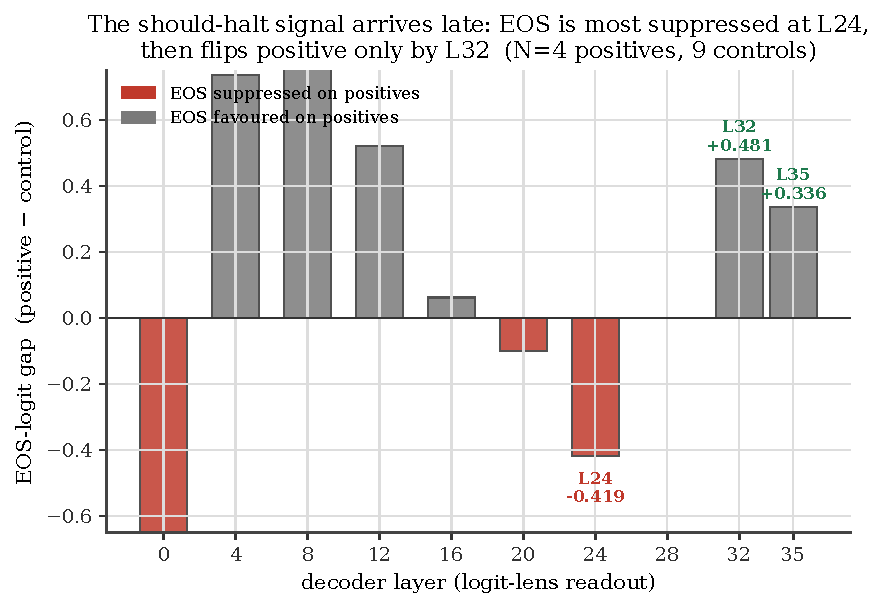
\includegraphics[width=0.85\linewidth]{fig_logit_lens_eos_gap.pdf}
  \caption{Logit-lens EOS-logit gap (positive minus control) by decoder layer. The gap
  is most negative at L24 ($-0.419$), meaning EOS is most suppressed there, then flips
  positive to $+0.481$ at L32 and $+0.336$ at L35. The should-halt signal becomes
  legible at the unembedding only in the final layers, after the continuation state is
  committed upstream ($N=4$ positives, 9 controls).}
  \label{fig:logit_lens}
\end{figure}

\subsection{EOS suppression is relative, not absolute}

A naive reading would be that the model \emph{crushes} EOS to a near-zero logit. The
data say otherwise. Per-step analysis of a single representative cap-hit document
(\texttt{docvqa\_srgb0228\_p2}, traced to a 3000-token cap rather than the paper-wide
12{,}000-token cap) shows the
chosen-token-minus-EOS raw logit margin has mean roughly 20.61 and median roughly 20.63
over the logged steps, with $P(\text{EOS})$ held to a mean of roughly $10^{-7}$, ranging
from about $10^{-5}$ at its highest down to $10^{-16}$ at its lowest.
Strikingly, the cap-hit document's mean EOS logit ($+10.76$) is actually \emph{higher}
than a single clean control's ($+10.07$, \texttt{docvqa\_fhxn0226\_p2}, which halts on
its own at 193 tokens). EOS is not absolutely suppressed; it is
out-competed. As with the attention signal below, this is an $N=1$-vs-$N=1$ trace and
we read it as illustrative rather than statistically established. Continuation tokens simply out-score it by about 20 logits, which is
enough to crush the EOS probability to a mean of roughly $10^{-7}$ (ranging from about
$10^{-5}$ down to $10^{-16}$ over the logged steps) while the EOS
logit itself stays comfortably positive (Figure~\ref{fig:eos_margin}).

\begin{figure}[ht]
  \centering
  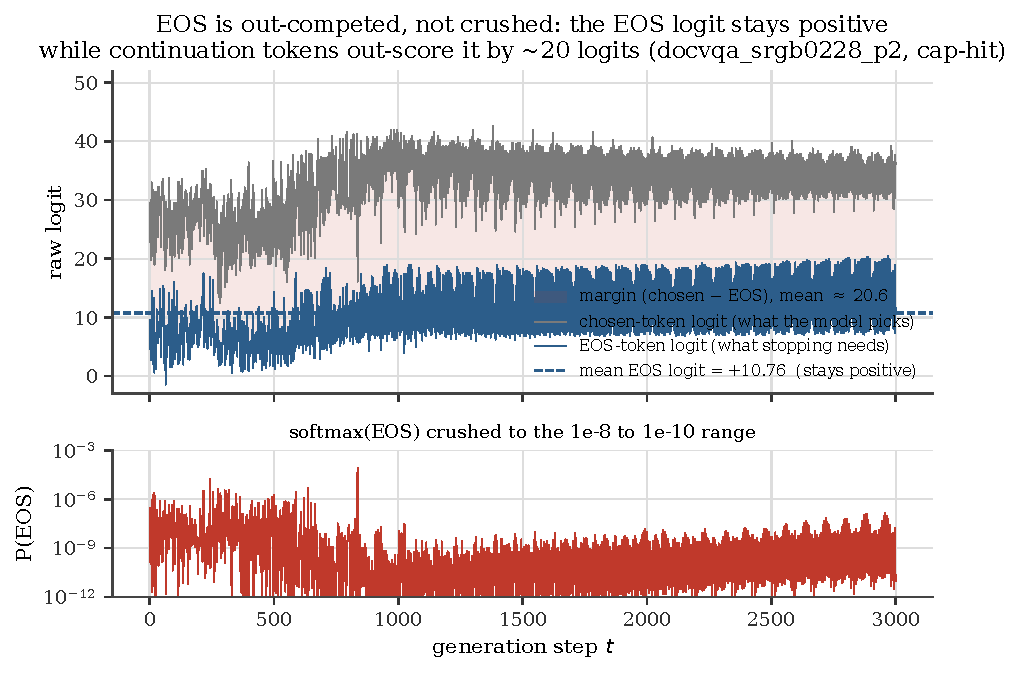
\includegraphics[width=0.85\linewidth]{fig_eos_relative_margin.pdf}
  \caption{EOS suppression is relative, not absolute (single cap-hit document
  \texttt{docvqa\_srgb0228\_p2}, 3000-token cap). The EOS logit
  stays positive throughout (mean $+10.76$, which actually exceeds a single clean control's
  $+10.07$), while continuation tokens out-score it by a mean margin of roughly 20.6
  logits, crushing $\mathrm{softmax}(\text{EOS})$ to a mean of roughly $10^{-7}$
  (ranging from about $10^{-5}$ down to $10^{-16}$). This is an $N=1$-vs-$N=1$ trace,
  shown as an illustration of the relative-suppression mechanism rather than as a
  powered comparison.}
  \label{fig:eos_margin}
\end{figure}

\subsection{Calibration is refuted: EOS is genuinely missing at loop onset}

If the failure were a near-miss in calibration, EOS would sit just below the argmax at
loop onset. It does not. The pooled record-level pool is $N=110$ loop-onset records,
but these are five contiguous records per document and are therefore pseudoreplicated;
we report the statistic at the document level (effective $N=22$ documents). Per document
the EOS token sits at a median rank of roughly 12{,}234, no document has its per-document
median rank inside the top 5, and only 1 of the 22 documents puts EOS in the top 5 at
\emph{any} logged onset position (the pooled record-level figures are a median rank of
roughly 10{,}502 and 0.9\% of records in the top 5). EOS is genuinely buried, not
narrowly under-promoted. We note a framing
caveat: programmatic n-gram loop-onset detection biases late, since records sit
thousands of tokens deep, so ``at loop onset'' is a late-onset operationalization.

\subsection{Coherent, not corrupted: the loop runs on a normal-norm residual}
\label{sec:normnull}

A leading competing account of degenerate generation is that the loop rides a
\emph{corrupted} residual state: an attention-sink / extreme-token regime in which a few
tokens accumulate anomalously large activations and the residual norm blows up
\citep{xiao2024streaming,repeatedtoken2025}. That mechanism makes a sharp, falsifiable
prediction about the residual L2 norm: once the loop is entered, the in-loop residual
norm should be \emph{much larger} than the pre-loop norm, with extreme-token reports
placing the inflation at $\gtrsim 3\times$ the surrounding-token norm. We measure the
residual L2 norm at the target layer (L24) inside versus outside the loop for the three
cap-hit documents and find the opposite: the loop runs on a residual that looks
\emph{normal}, not corrupted. The in-loop/pre-loop mean residual-norm ratio is
$0.96\times$ (\texttt{kshm0227\_p6}: mean norm $86.6$ in-loop vs.\ $90.0$ pre-loop),
$0.90\times$ (\texttt{srgb0228\_p2}: $84.0$ vs.\ $93.7$), and $0.97\times$
(\texttt{pgjw0227\_p5}: $84.3$ vs.\ $87.3$). In every case the norm \emph{shrinks
slightly} on entering the loop, and all three sit far below the $\geq 3.0\times$
inflation the attention-sink / extreme-token corruption mechanism requires. The
residual norm does not merely fail to grow with the halt score; it \emph{anti-correlates}
with it: the full-trace correlation between residual norm and the halt-direction
projection is negative for all three documents ($-0.24$, $-0.54$, $-0.30$). A larger
norm is associated with a \emph{more}-halt reading, not the runaway, never-halt
inflation a sink-corruption account would predict.

We read this as an affirmative null that rules out the attention-sink / extreme-token
corruption mechanism for our setting, rather than merely declining to find it. The loop
is not running on a blown-up, sink-dominated residual that has lost the information needed
to halt; it is running on a normal-looking residual whose halt-relevant projection is
miscomputed. The failure is a \emph{miscomputed decision on a coherent state}, not a
\emph{corrupted state}. This complements the relative-suppression and burial findings
above (the EOS logit stays positive, just out-scored) and converts the attention-sink
account from an untested competing hypothesis, mentioned only in passing in the related
work, into one we can affirmatively set aside here on the residual-norm evidence.
CAVEAT: this is an $N=3$ measurement, and the readout direction is itself
repetition-density-correlated (the modal per-document verdict is
``repetition-driven'': the full-trace correlation between repetition density and the
halt projection is $+0.84$, $+0.90$, $+0.74$), so the anti-correlation with norm is
consistent with, and does not escape, the repetition-density confound disclosed
elsewhere in this paper. The norm result discriminates against \emph{corruption}; it does
not by itself identify what the halt projection \emph{is} tracking.

% ===========================================================================
\section{Single-site fixes do not install halting: a converging series of nulls}
\label{sec:causal}
% ===========================================================================

If the deficit were a single localizable fault, the cheap fix would be to perturb one
site: install or abolish halting by adding, removing, or zeroing a single direction,
component, head, or layer. We tried this six ways and it does not work. Across six
converging perturbation experiments (single-direction project-out, component-resolved
patching, induction-head zeroing, prompt-engineering counterfactuals, SAE-feature
ablation, and multi-layer coordinated patching), all returning the pre-registered
FAIL/null verdict, no single-site intervention moves the token count. This is the
systems-relevant conclusion of the paper: you cannot patch one site to make it stop. We
flag at the outset what the nulls do and do not establish. They establish that single-
and multi-site perturbation does not install halting at this protocol's power. They do not
establish \emph{why}: a converging set of nulls is equally consistent with a genuinely
distributed deficit and with a protocol under-powered at the halt-relevant locus,
especially since three of the six rest on only $N=2$ documents. We do not adjudicate that
mechanistic question here (Section~\ref{sec:limitations}); the present section reports the
nulls and the one positive control that bounds, but does not eliminate, the under-powered
alternative.

\subsection{Sufficiency null at L0}

Injecting the class-matched bare-word-repeat halt direction at layer 0 does not induce
halt-failure. At the pre-registered target scale ($\alpha = 10$), the change in cap-hit
rate versus the vanilla run is 0.0 percentage points, against a pre-registered PASS
threshold of $\geq 40$ pp, a clear failure of the sufficiency hypothesis. Layer 0 is a
readout, not a generator.

\subsection{Norm-scaled positive control bounds, but does not eliminate, ``protocol under-powered''}

A reviewer might object that the perturbation protocol is simply too weak to move
anything. The norm-scaled positive control speaks to this, but only partially, and we
state its composition precisely because it is load-bearing. The run scaled a
single-direction layer-24 patch to $0.1\times$, $10\times$, and $100\times$ the
residual norm over four documents, but only \emph{three} of those were cap-hit
positives (manifest label \texttt{positive}: vanilla runs of $12{,}000$ tokens). On
those three positives, none escapes the cap at any scale; all stay pinned at
$12{,}000$. The perturbations nonetheless \emph{do} land visibly in the output (one
document gets a foreign-language token prepended, another gets stray Markdown emphasis
inserted), so the protocol is demonstrably not inert: it delivers content-altering
perturbations; it just cannot dislodge the halt-failure state. Content moves while
token count does not. The fourth document
(\texttt{table\_N005\_C04\_s05000}, manifest label \texttt{control}) was \emph{not} a
cap-hit positive (it halts cleanly on its own at 477 tokens with an EOS stop), and
so it cannot ``escape'' a cap it never hit. We flag it explicitly rather than fold it
into the positive tally, because under the same perturbation its output \emph{collapsed}:
to 3 tokens at $10\times$, to 1 token at $0.1\times$, and to $12{,}000$ tokens of
degenerate single-character repetition at $100\times$. That collapse is a norm-shock
signature; if anything it \emph{weakens} the protocol-sensitivity rebuttal, by showing
that this matched-norm patch can shatter a clean halt rather than cleanly perturb it, so
we do not count it as a positive. We are careful about what the three positives rule out.
They rebut the \emph{strongest} form of the under-powered objection (that the protocol
delivers no perturbation at all) but they do not rebut the weaker, more relevant form:
that the protocol cannot perturb the \emph{specific} halt-relevant direction at the
\emph{specific} halt-relevant locus. A random-direction patch that visibly reorders
surface tokens (or shatters an unrelated clean halt) is not evidence that a targeted
patch of the halt mechanism would have been detectable. We therefore treat the positive
control as a sensitivity floor, not as a clean refutation of under-power.

\subsection{The on-record null count, stated honestly}

Our strongest necessity test is a reverse-direction project-out experiment: it asks
whether \emph{removing} the halt direction, by projecting it out of the residual stream
at every position, lengthens generation. It does not. Across three clean-halting
controls the projected-out run is unchanged (within 10\%: $+9.1\%$, $0\%$, $0\%$), and
the positive document stays pinned at the cap, yielding a readout verdict. Importantly,
the project-out hook is confirmed to fire: two of the four documents produce materially
different output under it (one positive flips its table from Markdown to HTML), so this
is a genuine null and not a silently inert intervention (Figure~\ref{fig:b3_reverse}).

\begin{figure}[ht]
  \centering
  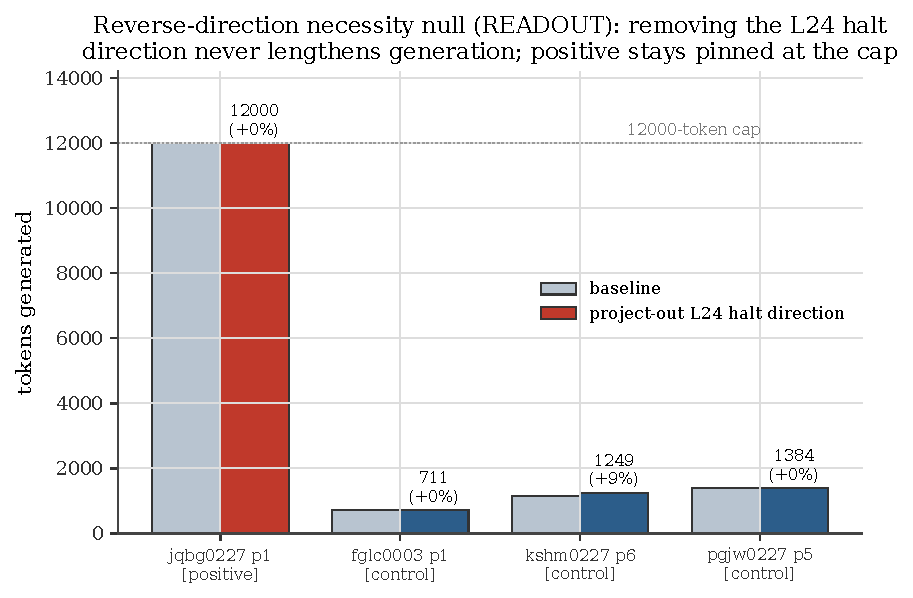
\includegraphics[width=0.85\linewidth]{fig_b3_reverse_direction.pdf}
  \caption{Reverse-direction necessity null (READOUT verdict). Projecting out the L24
  halt direction at every position does not lengthen generation: the positive document
  stays pinned at the 12000-token cap (12000 to 12000, $+0\%$) and the three
  clean-halting controls are unchanged ($+9.1\%$, $0\%$, $0\%$). The project-out hook is
  confirmed to fire (output content changes without length change), so this is a genuine
  null.}
  \label{fig:b3_reverse}
\end{figure}

A component-resolved patch grid points the same way. It decomposes the patch into MLP,
attention, and block contributions at layers 16, 20, and 24, across 5 documents and 4
intervention types: 0 of 45 real-patch cells produce any length reduction (a clean
real-null), while 9 of 134 control cells do (Figure~\ref{fig:p16_component}). The honest,
pre-registered caveat is sharper than off-layer norm-shock alone: only 4 of the 9 nonzero
controls are off-layer perturbations, while the remaining 5 fire \emph{at the same layer
and component as the real patch} (2 random-matched-norm, 3 shuffled-values). The clearest
warning sign is at L16/block\_output, where a random vector matched to the real patch's
norm ($\approx 47.4$) reduced one document's length by $99.95\%$ while the real
readout-direction patch at exactly that site reduced it by $0\%$. This makes ``the controls
themselves are suspect'' (the protocol's own perturbations can collapse generation in
ways unrelated to any halt direction) a live alternative reading, not merely off-layer
norm-shock, so the grid bounds protocol sensitivity rather than localizing a mechanism. The
verified positive control above is our best evidence that the protocol has real sensitivity.

\begin{figure}[ht]
  \centering
  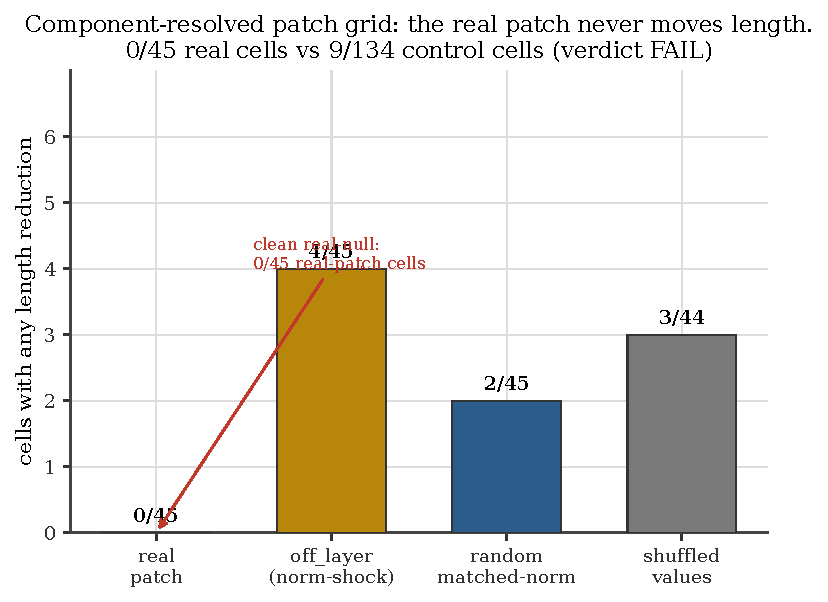
\includegraphics[width=0.85\linewidth]{fig_p16_component_grid.pdf}
  \caption{Component-resolved patch grid by intervention type. The real patch never
  moves length (0/45 cells, a clean real-null), while 9/134 control cells show a nonzero
  reduction: 4 off-layer, 2 random-matched-norm, and 3 shuffled-values. Only 4 are
  off-layer; the other 5 fire at the same layer and component as the real patch. Most
  starkly, at L16/block\_output a random vector matched to the real patch's norm
  ($\approx 47.4$) cuts one document's length by $99.95\%$ while the real patch there
  cuts $0\%$. Verdict FAIL. These nonzero controls make ``the controls are suspect'' a
  live reading and bound protocol sensitivity rather than localizing a mechanism.}
  \label{fig:p16_component}
\end{figure}

Accordingly, our load-bearing causal evidence is \emph{six converging perturbation nulls},
all returning the pre-registered FAIL/null verdict, with $N$ ranging from 2 to 22
documents. We are precise about provenance: the two anchor nulls (B3 and P16) are
verified on disk in this repository; the other four (P10b, P19, P12, and P22) are recorded
with their pre-registered FAIL verdicts and their primary summary files are pending
re-sync for external release. The six are:

{\sloppy
\begin{enumerate}
  \item \textbf{B3, reverse-direction project-out null} (necessity; READOUT verdict; 3/3
  controls unchanged, positive pinned at the cap, project-out hook confirmed to fire;
  \texttt{p2\_pilot/b3\_reverse\_direction\_summary.json});
  \item \textbf{P16, component-resolved patch grid} (necessity; FAIL verdict; 0/45
  real-patch cells reduce length, 9/134 control cells do, $N=5$ documents;
  \texttt{p16\_component\_resolved\_short/\_summary.json}). P16 subsumes the earlier
  component claims CL-19 and CL-20 and is counted once here, not as two separate nulls;
  \item \textbf{P10b, induction-head zeroing} (necessity; FAIL verdict; 0/4 induction
  heads pass the pre-registered 30\% threshold under zeroing, $N=2$ documents;
  \texttt{p10b\_head\_zero\_patching/\_summary.json});
  \item \textbf{P19, system-prompt counterfactual} (FAIL verdict; 0/6 stop-instruction
  prompts pass, median reduction 0\%, $N=5$ documents;
  \texttt{p19\_system\_prompt\_counterfactual/\_summary.json});
  \item \textbf{P12, SAE-feature ablation} (FAIL verdict; 0/5 cross-validation folds pass
  all pre-registered criteria, top-feature AUC 0.54 to 0.63 against a 0.85 bar, $N=22$
  positives versus 56 controls; \texttt{p12\_sae\_ablation/\_summary.json});
  \item \textbf{P22, multi-layer coordinated patch} (FAIL verdict; the real coordinated
  zero-patch of the L16/L20/L24 window reduces length 0\%, $N=2$ documents;
  \texttt{p22\_multilayer\_coordinated/\_summary.json}).
\end{enumerate}
\par}

These six are independent perturbation classes (project-out of a single direction,
forward-patching of resolved components, head-level zeroing, prompt-level counterfactuals,
SAE-feature ablation, and a multi-layer coordinated patch), and each carries its own
positive or control evidence, so they are not a single test reported six times. We keep the
count honest in both directions. On provenance: B3 and P16 are verified on disk, while
P10b, P19, P12, and P22 are recorded with their FAIL verdicts and primary files pending
re-sync, so the load-bearing local anchors are the first two. On power: three of the six
rest on small samples ($N=2$ for B3's positive, P10b, and P22), and a uniform null at small
$N$ does not by itself separate a genuinely distributed deficit from an under-powered
protocol (Section~\ref{sec:limitations}). We also carry the controls-are-suspect caveat
openly: in the component grid, 5 of the 9 nonzero controls fire at the same layer and
component as the real patch (not merely off-layer), and a norm-matched random vector
($\approx 47.4$, the real patch's norm) reduced one document's length by $99.95\%$ at
L16/block\_output where the real readout-direction patch reduced $0\%$. That a matched-norm
random perturbation collapses generation where the real patch does nothing makes ``the
controls themselves are suspect'' a live alternative to ``the protocol is under-powered,''
rather than a simple off-layer norm-shock artifact.

We state the bottom line for this section plainly, because it is the load-bearing systems
conclusion of the paper. All single- and multi-site perturbations we ran returned null at
this protocol's power: you cannot patch one site to make the model stop, so the deficit is
not a single steerable fault. Whether the underlying deficit is genuinely distributed or
the protocol is simply under-powered at the halt-relevant locus is \emph{not resolved} by
these data, and we do not need to resolve it for the systems claim. The discriminating
experiment (a positive-control patch of the \emph{same} readout direction at a
\emph{non-loop} position, which would separate ``distributed'' from ``under-powered'') is
left to the companion representational-geometry paper and to future work.

% ===========================================================================
\section{Cross-family: motivation only}
\label{sec:crossfamily}
% ===========================================================================

To motivate that this is not one fine-tune's idiosyncratic bug, we ran a small
$4 \times 4$ document-by-model grid spanning four model families (SmolDocling-256M-preview,
InternVL3-8B, Qwen3-VL-8B-Instruct, and Qwen3-VL-30B-A3B-Instruct) crossed with four
documents. Under a strict criterion (\texttt{stop\_reason == max\_new\_tokens}), halt-failure
reproduces on 10 of the 16 cells, with at least one cap-hit cell in every family (per-family
3/4, 1/4, 3/4, 3/4); a more permissive near-cap relabel raises the tally to 11/16, so the
count is criterion-dependent. Sixteen cells over four families is far too thin to support a
generality claim, and the directory-level aggregate verdict over this run abstains
(\texttt{INSUFFICIENT\_DATA}). We therefore use this only as a motivation that the
phenomenon is not unique to the studied fine-tune, and defer any actual generality claim to
a dedicated companion note that owns the cross-family matrix.

% ===========================================================================
\section{The deployable artifact: a runtime monitor and its honest trade-off}
\label{sec:production}
% ===========================================================================

The deliverable is a runtime monitor that reads the layer-24 readout direction at the
early site identified in Section~\ref{sec:early_commitment} and boosts the EOS logit when
the readout fires. It suppresses runaway generation, but it sits on a genuine
precision-recall trade-off rather than a free lunch, and there is no free sweet spot.

At a $+6.91$ EOS boost, the reactive monitor achieves a 37.68\% mean length reduction
with 0 of 10 control false-positives and 5 of 13 positive cap-hits remaining
(Figure~\ref{fig:monitor_tradeoff}). This is the deployable clean-specificity operating
point. At a $+30$ EOS boost, the same monitor achieves a 99.58\% mean length reduction
with 0 remaining cap-hits, but at a catastrophic 10 of 10 control false-positives. The two
operating points bracket the trade-off: you can buy near-total loop suppression only by
destroying clean-document specificity, so the deployable point is the conservative $+6.91$
boost. We are explicit about the scope of the false-positive bound: the 0-of-10 figure is
measured on $N=10$ clean controls, a workshop-scale specificity check, not a large-corpus
false-positive rate. Characterizing the false-positive rate at the $N \geq 600$ long-form
scale a production deployment would require is left to future work; the present claim is a
small-$N$ specificity bound, not a deployment-grade FP guarantee.

\begin{figure}[ht]
  \centering
  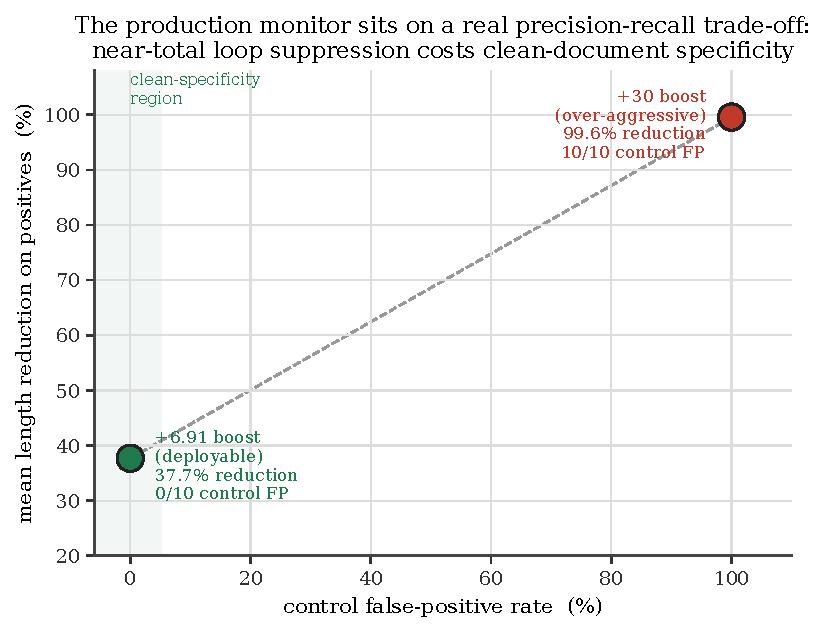
\includegraphics[width=0.85\linewidth]{fig_monitor_tradeoff.pdf}
  \caption{The production monitor sits on a real precision-recall trade-off. At a
  $+6.91$ EOS boost it gives 37.7\% mean length reduction with 0/10 control
  false-positives (deployable clean-specificity point); at a $+30$ boost it gives 99.6\%
  reduction with 0 remaining cap-hits but 10/10 control false-positives. Near-total loop
  suppression costs clean-document specificity. $N=13$ positives, 10 controls.}
  \label{fig:monitor_tradeoff}
\end{figure}

\paragraph{Image content is sufficient to sustain the loop.}
Replacing the input image with grey noise collapses every tested cap-hit positive from a
full-cap runaway to a short clean-EOS halt: across the tested positives, baseline
cap-length stops become 13- to 18-token, EOS-terminated halts under grey-noise inpaint.
All 5 of 5 explicitly named positives collapse this way (\texttt{arxiv\_table\_000266},
\texttt{docvqa\_jqbg0227\_p1}, \texttt{docvqa\_kshm0227\_p7}, \texttt{docvqa\_srgb0228\_p2},
\texttt{funsd\_105\_105}); with $N=5$ we report the count qualitatively rather than
attaching a Wilson interval. We state the claim as image \emph{content} being sufficient
to sustain the loop rather than as a clean vision-causality demonstration, because
grey-noise replacement confounds removing visual evidence with destroying readable
content; the discriminating experiment (swapping in a different readable document) is left
to future work. This still motivates a vision-aware guardrail rather than a purely
text-side penalty: the halt-failure state is conditioned on the visual input.

A correlational vision signal points the same way. In a single-positive-versus-single-control
comparison, the positive document's text-to-image attention mass collapses in the L20 to
L24 halt band: the positive-to-control ratio is 0.070 at layer 20 ($14.2\times$ lower),
0.216 at layer 24 ($4.6\times$ lower), and only a modest 0.695 at layer 16. The collapse
is band-localized rather than monotone: the \emph{same} document pair shows the positive
with \emph{higher} image attention than the control at layer 8 ($1.10\times$) and again at
layer 35 ($1.37\times$), so the L20-to-L24 dip is suggestive only. We flag this
as $N=1$-vs-$N=1$ and reserve it for future larger-sample work.

% ===========================================================================
\section{Related work}
\label{sec:related}
% ===========================================================================

Our work sits at the intersection of seven threads: language-model degeneration,
hallucination in vision-language models (VLMs), the mechanistic-interpretability
toolkit, single-direction steering, the geometry of count-and-halt decisions,
attention-sink accounts of termination, and cross-modal grounding collapse. We review
each and locate our contribution against it.

\paragraph{Degeneration, repetition, and non-termination.}
Failure to terminate is a long-standing pathology of likelihood-trained autoregressive
decoders: likelihood decoding produces bland, repetitive, degenerate text
\citep{holtzman2020degeneration}, and greedy, beam, top-$k$, and nucleus decoding are all
provably inconsistent, able to emit infinite-length, zero-probability sequences unless
the model is made self-terminating \citep{welleck2020consistency}. The training objective
has itself been implicated, motivating unlikelihood training to suppress repetition at the
source \citep{welleck2019unlikelihood}. In production OCR pipelines the symptom is acute
enough to be engineered around directly: retry mechanisms and post-hoc filters are now
standard \citep{poznanski2025olmocr,olmocrv2}, and repetition is documented as a
first-class production concern in both general LLM serving
\citep{repetitionproduction2025} and recent VLM releases \citep{internvl35}. These works treat non-termination as a symptom
to be suppressed at the decoding or serving layer rather than as a representational
phenomenon to be localized. A complementary, mechanistically-flavored line asks
\emph{why} the decoder loops. The repeated-token phenomenon has been interpreted at the
level of early-layer attention and sink structure \citep{repeatedtoken2025}, and
single-neuron and single-head accounts of repetitive generation exist for text-only
models: ``repetition neurons'' identify neuron-level circuits that drive repeats
\citep{repetitionneurons2025}, while induction-head accounts trace pattern completion to
match-and-copy heads \citep{olsson2022induction} and quantify when those heads over-fire
on repeated context \citep{wang2025inductiontoxicity} (note: this preprint was withdrawn in December 2025). These are the closest causal
hypotheses to ours, and we situate against them deliberately. They are perpendicular on
three axes: they study text-only LLMs rather than fine-tuned OCR-VLMs, they target
repetition as such rather than the broader \emph{halt-failure} phenomenon (of which
token loops are one surface class among several, including phantom table rows and
structural-marker hallucination), and they localize repetition to single neurons or
heads (and, where intervened, report that ablating or regularizing them changes
behavior). Our central systems finding is the opposite: a converging series of
single-direction and single-layer perturbations \emph{fails} to move the token count,
which is why we conclude that single-site fixes do not install halting (whether the
underlying deficit is genuinely distributed is taken up in the companion paper).

\paragraph{Hallucination in (V)LMs, including structural and OCR hallucination.}
Most VLM hallucination research concerns object hallucination in captioning and VQA, as
captured by benchmarks such as POPE \citep{li2023pope} and surveyed broadly in
\citet{bai2024mllmhallusurvey}. Document OCR introduces a distinct, \emph{structural}
failure mode: phantom blank table rows, fabricated page numbers and watermarks, and
runaway markup loops; the closest mitigation-side work studies OCR hallucination under
degraded input on the same model family with a dedicated benchmark and an
uncertainty-aware fix \citep{he2025seeingbelieving}. We study this on a fine-tune of the
Qwen2.5-VL family \citep{qwen25vl}; the same surface symptoms recur across OCR-VLM releases
\citep{poznanski2025olmocr,olmocrv2,internvl35,granitedocling2025}. The mechanistic
substrate for OCR-specific behavior has begun to be mapped: text-inpaint causal
protocols localize where OCR information enters the residual stream
\citep{steinberggal2026}, and path-patching studies isolate vision-to-text ``OCR heads''
that route visual evidence into the language stream \citep{baek2025}. We borrow the
text-inpaint logic for our image-content test, where replacing the input image with
grey noise collapses tested cap-hit positives (all 5 of 5 named documents) from
12{,}000-token runaways into short \texttt{stop\_reason=eos} halts of 13 to 18 tokens,
establishing that image content is sufficient to sustain the halt-failure state (we say
``sufficient'' rather than ``causally load-bearing'' because grey noise confounds removing
visual evidence with destroying readable content). Where these works localize \emph{where OCR
content arrives}, we ask \emph{where and when the runaway becomes detectable} and show that
the decision to terminate is missing rather than mislocated at a single routing site.

\paragraph{Mechanistic-interpretability methods.}
Our diagnostics are a small subset of the standard mechinterp toolkit. We fit linear
probes \citep{alain2016probes} for early detection of the cap-hit outcome, and we
triangulate the depth at which a ``should-halt'' signal becomes legible at the unembedding
using the logit lens \citep{nostalgebraist2020logitlens} and its better-calibrated
tuned-lens variant \citep{belrose2023tunedlens}; this is what surfaces our minimal depth
fact that the EOS logit gap is most negative at L24 and only flips positive by L32, i.e.,
the should-halt signal arrives too late to override an already-committed continuation
state. Our perturbation tests use activation and path patching in the lineage of
causal-mediation and circuit-level analysis \citep{meng2022rome,wang2023ioi}, including
component-resolved causal tracing \citep{fcct2025} and SAE-feature ablation
\citep{bricken2023monosemanticity,saelens2024,park2025save}, all implemented as direct
PyTorch forward hooks following the intervention-API conventions of
\citep{pyvene2024,nnsight2024}. The deeper representational diagnostics that these methods
also enable (per-class halt-direction geometry, build-versus-read decomposition, and a
base-versus-fine-tune crosscoder comparison \citep{dfc2025} showing the geometry is
fine-tune-introduced) are reported in the companion representational-geometry paper rather
than here. The ``readout-versus-locus'' distinction we draw at L24 shares its mechanism
vocabulary with hallucination-detection work that reads model internals
\citep{redeep2024}.

\paragraph{Single-direction and steering methods.}
The hypothesis that a behavior lives along a single residual-stream direction, testable
by adding or projecting out that direction, is most cleanly stated for refusal, which is
mediated by a single direction recoverable and steerable across many chat models
\citep{arditi2024refusal}, and has a direct method-class ancestor in inference-time
intervention, which steers along an attention-head truthfulness direction
\citep{li2023iti}; the underlying add-a-difference-vector mechanism is the activation-engineering
recipe our injections instantiate \citep{turner2023activationengineering}. That
single-direction picture is itself contested: refusal has been shown to factor into
geometrically distinct, class-specific directions rather than one universal steerable axis
\citep{joad2026morethanrefusal}, a class-specific picture the companion paper develops for
halt directions. Our production monitor is the OCR-halt analogue of these methods: it reads
an L24 readout direction and boosts the EOS logit rather than shifting an activation. The
closest VLM-side comparable performs decoder-time steering pre-decoding rather than via a
mid-decoder forward hook \citep{steervlm2025}, and class-conditional steering offers a
finer-grained alternative when one global direction is too coarse \citep{yin2026dmas}.
Crucially, our single-direction tests come back null. Injecting a class-matched halt
direction at L0 changes the cap-hit rate by 0.0 percentage points against a pre-registered
40-point PASS threshold, and a norm-scaled positive control fails to dislodge the halt
state at $0.1\times$, $10\times$, or $100\times$ the residual norm (0 of 3 cap-hit
positives escape the cap at any scale; a fourth, clean-halt control in the same run instead
collapsed under the patch) even though the perturbations visibly alter output content. This
is the inverse of the steering-success narrative in the single-direction literature: the
readout is \emph{decodable} without being \emph{steerable}. We read this
decodable-but-not-steerable gap as the systems statement that single-site fixes do not
install halting, while noting it is equally consistent with a protocol under-powered at the
halt-relevant locus; we do not adjudicate between the two (Section~\ref{sec:limitations}).

\paragraph{The counting-manifold account of halt decisions.}
The decision to stop is, in part, a decision about \emph{how much} has been emitted, which
connects halt-failure to the geometry of counting, where a running count is tracked along a
low-dimensional curved manifold and used to make a stop-or-continue decision
\citep{gurnee2026countmfd}; the companion representational-geometry paper takes up whether a
count-manifold and build-versus-read offset organize the halt signals, which is out of
scope for this systems paper.

\paragraph{Attention sinks, EOS-halting, and SinkTrack.}
A prominent family of accounts ties termination and long-context stability to attention
sinks. The attention-sink phenomenon was first identified on the initial tokens of a
sequence and exploited for stable infinite-length streaming generation
\citep{xiao2024streaming}. Building on it, SinkTrack treats an anchor token as an
information sink and injects context into it to counteract attention drift, reporting
multimodal gains \citep{sinktrack2026}, and the repeated-token failure has itself been
traced to attention-sink structure \citep{repeatedtoken2025}. This is the most actionable
competing mechanism for our setting
and a natural baseline. Our evidence is only partly aligned with it: we find that EOS
suppression is \emph{relative, not absolute}, with continuation tokens out-scoring EOS by
roughly 20 logits while the EOS logit itself stays positive (in a single $N=1$-vs-$N=1$
trace a cap-hit document's mean
EOS logit of $+10.76$ exceeds a clean control's $+10.07$), and that at loop
onset EOS is genuinely buried (per-document median rank near 12{,}000 over 22 documents,
only 1 of which ever puts EOS in the top 5), rather than narrowly
under-promoted by a single mis-set sink. More directly, we test the residual-norm
prediction this account makes, a $\gtrsim 3\times$ in-loop norm inflation, and find
the opposite (Section~\ref{sec:missinghalt}): the in-loop/pre-loop residual norm is
$0.96\times$/$0.90\times$/$0.97\times$ across the three cap-hit documents, far below the
$\geq 3.0\times$ corruption regime, and the norm anti-correlates with the halt score. The
loop runs on a normal-norm, coherent residual, so we read the failure as a miscomputed
decision rather than a sink-corrupted state, and we affirmatively set the
attention-sink / extreme-token corruption mechanism aside for our setting (at $N=3$, with
the repetition-density confound noted). A sink-anchoring intervention is therefore a
complement to, not a substitute for, the missing-halt-signal reading.

\paragraph{Cross-modal grounding collapse.}
Finally, several works frame VLM hallucination as a drift of attention away from visual
evidence toward linguistic priors. Visual contrastive decoding contrasts outputs from
original versus distorted images to suppress over-reliance on language priors
\citep{leng2024vcd}, and a complementary line reorients attention toward image tokens at
the moment grounding is needed: confidence-aware attention calibration rescales attention
to counter late-generation modality drift \citep{fazli2025caac}, and attention-lens
analyses diagnose text-vs-vision routing as the locus of modality bias and rebalance the
two streams \citep{zheng2025modalitybias}. This ``detect the decision moment, then
intervene'' structure matches our production setting, and the modality-bias account is
corroborated on our side by a (single-positive-versus-single-control, hence preliminary)
collapse of text-to-image attention mass in the L20 to L24 band.

\paragraph{Positioning.}
Against all of these, our systems contribution is to read OCR-VLM halt-failure not as a
single broken layer, sink, head, or steerable direction, but as a \emph{missing halt
signal}: a should-halt signal that exists yet arrives too late and is out-competed, running
on a coherent (not corrupted) residual, robust to single-site perturbation in both the
necessity and sufficiency directions, and conditioned on the visual input. On that reading
we build the deliverable, a runtime readout monitor with an honest precision-recall
trade-off rather than a clean single-direction fix, and we treat the converging nulls as
first-class evidence that single-site fixes do not install halting. The representational
geometry that organizes the per-class halt signals (and the attractor hypothesis it
supports) is the subject of the companion representational-geometry paper, not this one.

% ===========================================================================
\section{Limitations and walk-back}
\label{sec:limitations}
% ===========================================================================

We state the walk-backs plainly because they are part of the contribution.

\begin{enumerate}
  \item \textbf{``Distributed'' is not resolved against ``under-powered,'' and we do not
  need to resolve it.} All single- and multi-site perturbations we ran returned null at this
  protocol's power, and whether the underlying deficit is genuinely distributed across many
  directions or the protocol is simply under-powered at the halt-relevant locus is not
  resolved by these data. The two readings are observationally equivalent at this protocol
  power. This is acceptable for the present paper because our claim is the systems one, that
  single-site fixes do not install halting, not the mechanistic one that the deficit is
  distributed. The experiment that would settle it (a positive-control patch of the same
  readout direction at a non-loop position) is left to the companion representational paper
  and to future work.

  \item \textbf{Necessity evidence is six converging nulls, but provenance and $N$ are
  uneven.} Six perturbation nulls all return the pre-registered FAIL/null verdict: the
  reverse-direction project-out null (B3, readout verdict, controls unchanged, positive
  pinned at the cap, project-out hook confirmed to fire), the component-resolved patch grid
  (P16, 0 of 45 real-patch reductions, $N=5$), induction-head zeroing (P10b, 0 of 4 induction
  heads pass under zeroing, $N=2$), the system-prompt counterfactual (P19, 0 of 6
  stop-instruction prompts pass, $N=5$), SAE-feature ablation (P12, 0 of 5 folds pass all
  criteria, top-feature AUC 0.54 to 0.63 versus a 0.85 bar, $N=22$ positives), and a
  multi-layer coordinated zero-patch (P22, real coordinated patch reduces length 0\%, $N=2$).
  On provenance: B3 and P16 are verified on disk in this repository; P10b, P19, P12, and P22
  are recorded with their FAIL verdicts but their primary summary files are pending re-sync
  before external release, so the two anchor nulls carry the local load. On power: three of
  the six rest on small samples (B3's positive document, P10b, and P22 each at $N=2$), and a
  uniform null at $N=2$ does not on its own discriminate a distributed deficit from an
  under-powered protocol; that disambiguation (item~1 above) remains open. The residual
  caveat is sensitivity, not verification: in the P16 grid 5 of the 9 nonzero control patches
  fire at the same layer and component as the real patch (only 4 are off-layer), so the six
  nulls establish ``single- and multi-site perturbation does not install halting at this
  protocol's power,'' not a fully exhaustive causal search.

  \item \textbf{The controls are suspect, and the positive control only bounds under-power.}
  In the component grid, a norm-matched random vector ($\approx 47.4$) cut one document's
  length by $99.95\%$ at L16/block\_output where the real readout-direction patch cut $0\%$,
  and 5 of the 9 nonzero controls are not off-layer. That matched-norm random perturbations
  can collapse generation where the real patch does nothing means ``the controls are
  suspect'' is a real alternative to ``the protocol is under-powered.'' Our verified positive
  control (Section~\ref{sec:causal}) is the load-bearing sensitivity evidence, but it rebuts
  only the strongest form of the under-powered objection (the protocol is not inert; it
  visibly alters content). It does not rebut the weaker, more relevant form, that the
  protocol cannot perturb the specific direction at the specific halt-relevant locus, which
  is why item~1 above remains open.

  \item \textbf{Cross-family reproduction is small-matrix and the aggregate verdict abstains.}
  Under the strict \texttt{stop\_reason == max\_new\_tokens} criterion, halt-failure reproduces
  on 10 of 16 doc-model cells across four families (per-family 3/4, 1/4, 3/4, 3/4), but the
  matrix is only sixteen cells and the directory-level aggregate verdict over this run is
  \texttt{INSUFFICIENT\_DATA}. We make no strong generality claim from it. A permissive near-cap
  relabel would shift the tally to 11/16, so the count is criterion-dependent. We use it as
  motivation only and defer a properly powered cross-family study to a companion note.

  \item \textbf{The monitor and image-inpaint results are workshop-$N$.} The monitor
  trade-off rests on $N=13$ positives and $N=10$ controls, and the image-inpaint result on
  $N=5$ named positives. The 0-of-10 false-positive figure is therefore a small-$N$
  specificity bound, not a deployment-grade false-positive rate; characterizing the FP rate
  at the $N \geq 600$ long-form scale a production deployment would require is future work.

  \item \textbf{The vision-attention-collapse signal is $N=1$-vs-$N=1$ and non-monotone.} The
  attention-collapse comparison is a single-positive-versus-single-control measurement,
  not yet statistically meaningful, and the band-localized L20-to-L24 dip is suggestive
  only: the same document pair shows the positive with \emph{higher} image attention than
  the control at L8 ($1.10\times$) and L35 ($1.37\times$). It is reserved for future
  larger-sample work.

  \item \textbf{Loop-onset framing biases late, and the calibration pool is clustered.} The
  calibration result is computed at programmatically detected onset positions that sit
  thousands of tokens deep; this overstates ``onset'' and is a framing concern, though it
  does not change the numeric finding that EOS is genuinely missing. The 110 onset records
  are five contiguous records per document and so are pseudoreplicated; we therefore report
  the statistic at the document level (effective $N=22$), where no document has a median
  EOS rank inside the top 5 and only 1 of 22 puts EOS in the top 5 at any logged position.
\end{enumerate}

% ===========================================================================
\section{Conclusion}
\label{sec:conclusion}
% ===========================================================================

Halt-failure in a fine-tuned OCR-VLM is best read, from a systems standpoint, as a
\emph{missing halt signal} rather than a single broken layer, a corrupted state, or mere
repetition. The supporting facts are pre-registered and converging: the network computes a
downstream should-halt signal that arrives too late to override an upstream continuation
state (logit-lens EOS gap $-0.419$ at layer 24 flipping to $+0.481$ by layer 32); that
suppression is relative not absolute (chosen-vs-EOS margin about 20 logits; an $N=1$
illustration); EOS is genuinely missing at loop onset (per-document median rank roughly
12{,}234 over 22 documents, only 1 of which ever puts EOS in the top 5); the loop runs on a
coherent, not corrupted residual (in-loop/pre-loop norm $0.90$ to $0.97\times$, ruling out
the $\geq 3\times$ inflation a sink-corruption account requires; $N=3$); and six converging
single-direction, single-layer, and multi-layer perturbations fail to move the token count.
On that last point we are deliberately careful: whether the underlying deficit is genuinely
distributed or the protocol is under-powered at the halt-relevant locus is \emph{not
resolved} by these data, and we do not need to resolve it for the systems claim that
single-site fixes do not install halting. Our load-bearing causal evidence is six converging
perturbation nulls, all returning the pre-registered FAIL/null verdict ($N$ ranging 2 to 22
documents): B3 and P16 are verified on disk, while P10b, P19, P12, and P22 are recorded with
their FAIL verdicts and their primary files pending re-sync. Three of the six rest on $N=2$,
and a uniform null at small $N$ does not by itself separate ``distributed'' from
``under-powered.'' The surface symptom is not unique to the studied fine-tune: under a
strict stop-reason criterion halt-failure reproduces on 10 of 16 doc-model cells across four
model families (11 of 16 under a permissive relabel), but the matrix is small and the
aggregate verdict abstains, so we use it as motivation only. The deliverable is a deployable
runtime readout monitor with an explicit precision-recall trade-off (37.68\% mean reduction
with 0 of 10 control false-positives but still leaving 5 of 13 positives at the cap, or
99.58\% reduction at 10 of 10 control false-positives), reading the layer-24 readout at the
early-commitment site, plus an image-inpaint result showing that image content is sufficient
to sustain the loop (all 5 of 5 named positives collapse to short EOS halts under grey
noise), which motivates a vision-aware guardrail. The walk-backs are part of the result:
showing where the single-cause story fails is what justifies treating the deficit as a
missing halt signal and shipping an honest trade-off rather than a clean single-direction
fix. The representational geometry that explains \emph{why} the per-class halt signals are
organized as they are, and the attractor hypothesis it supports, is the subject of a
companion representational-geometry paper.

% ===========================================================================
\bibliographystyle{plainnat}
\bibliography{references}
% ===========================================================================

\end{document}
